\chapter{Results \& Analysis}
\label{chapter:results}
\section{Results}
The circuit schematica was captured and simulated using the LTSpice software. The simulation was performed to analyze the performance of the circuit and to verify its functionality. The results of the simulation are presented in this section.
The simulation was performed using the following parameters:
\begin{itemize}
    \item Supply voltage: 1.8V
    \item Input frequency: 5MHz
    \item Input amplitude: 1.8V
    \item Frequency Multiplication Factor: 8
\end{itemize}
The simulation results are shown in the following figures. The first figure shows the 
output waveform of the circuit.output waveform of the circuit, which is a square wave. The output waveform is shown in Figure \ref{fig:output_waveform}.
\begin{figure}[H]
    \centering
    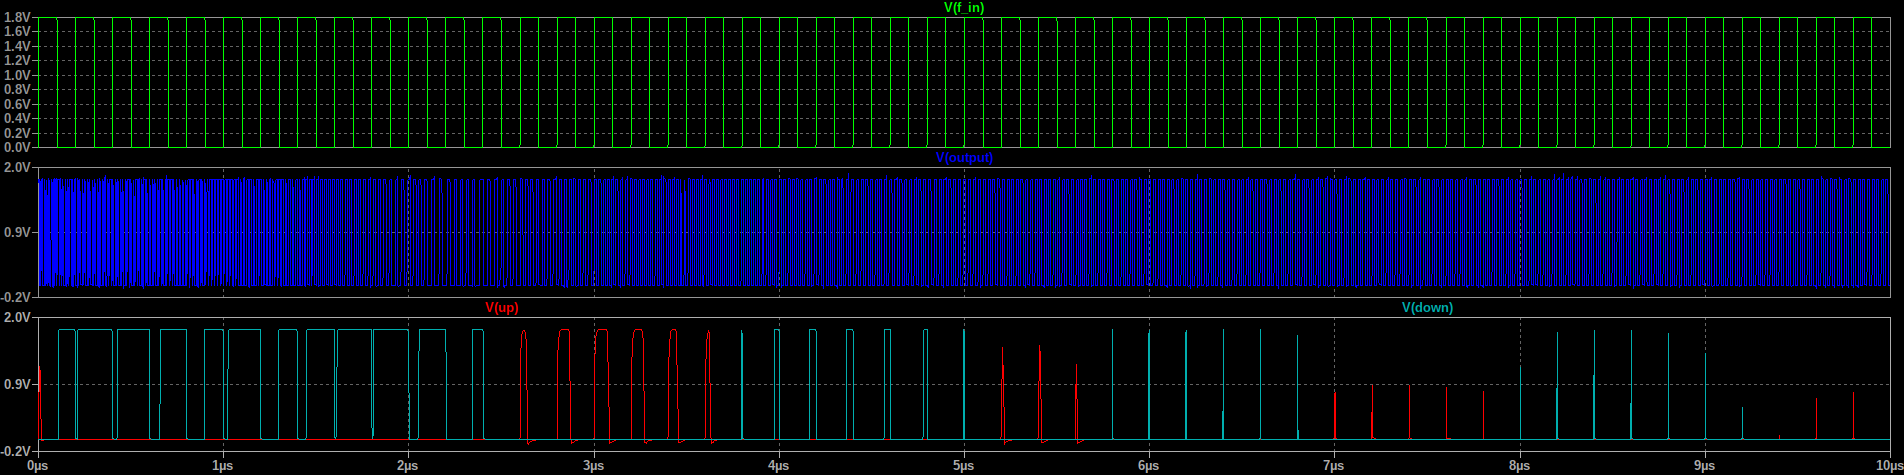
\includegraphics[width=1\textwidth]{figs/finalop5MHz.png}
    \caption{Output Waveform of PLL}
    \label{fig:output_waveform}
    \vspace{0.5cm}
\end{figure}
We can observe the phase locking of the output waveform with the input waveform in the Figure \ref{fig:output_waveform_phaselocking}.
\begin{figure}[H]
    \centering
    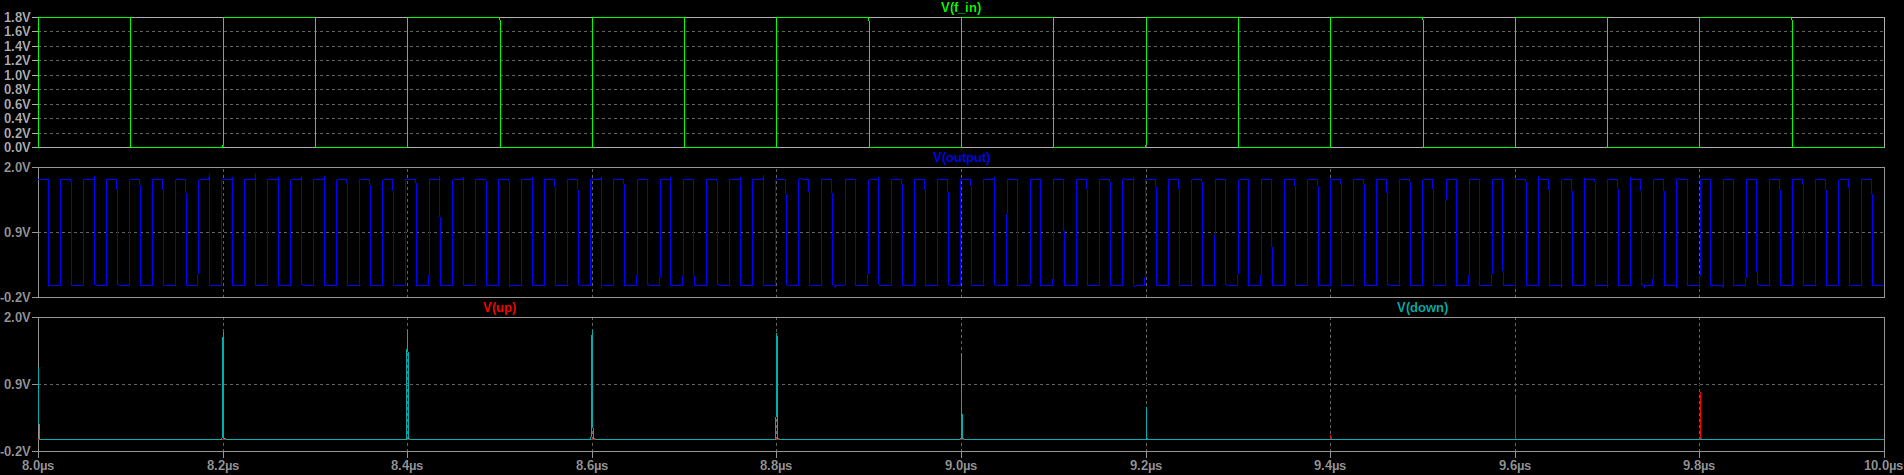
\includegraphics[width=1\textwidth]{figs/finalopphaselock.png}
    \caption{Magnified Output Waveform of PLL}
    \label{fig:output_waveform_phaselocking}
    \vspace{0.5cm}
\end{figure}
The second figure shows the output frequency spectrum of the circuit. The output frequency spectrum is shown in Figure \ref{fig:output_frequency_spectrum}. The output frequency spectrum shows the frequency components of the output waveform.

\begin{figure}[H]
    \centering
    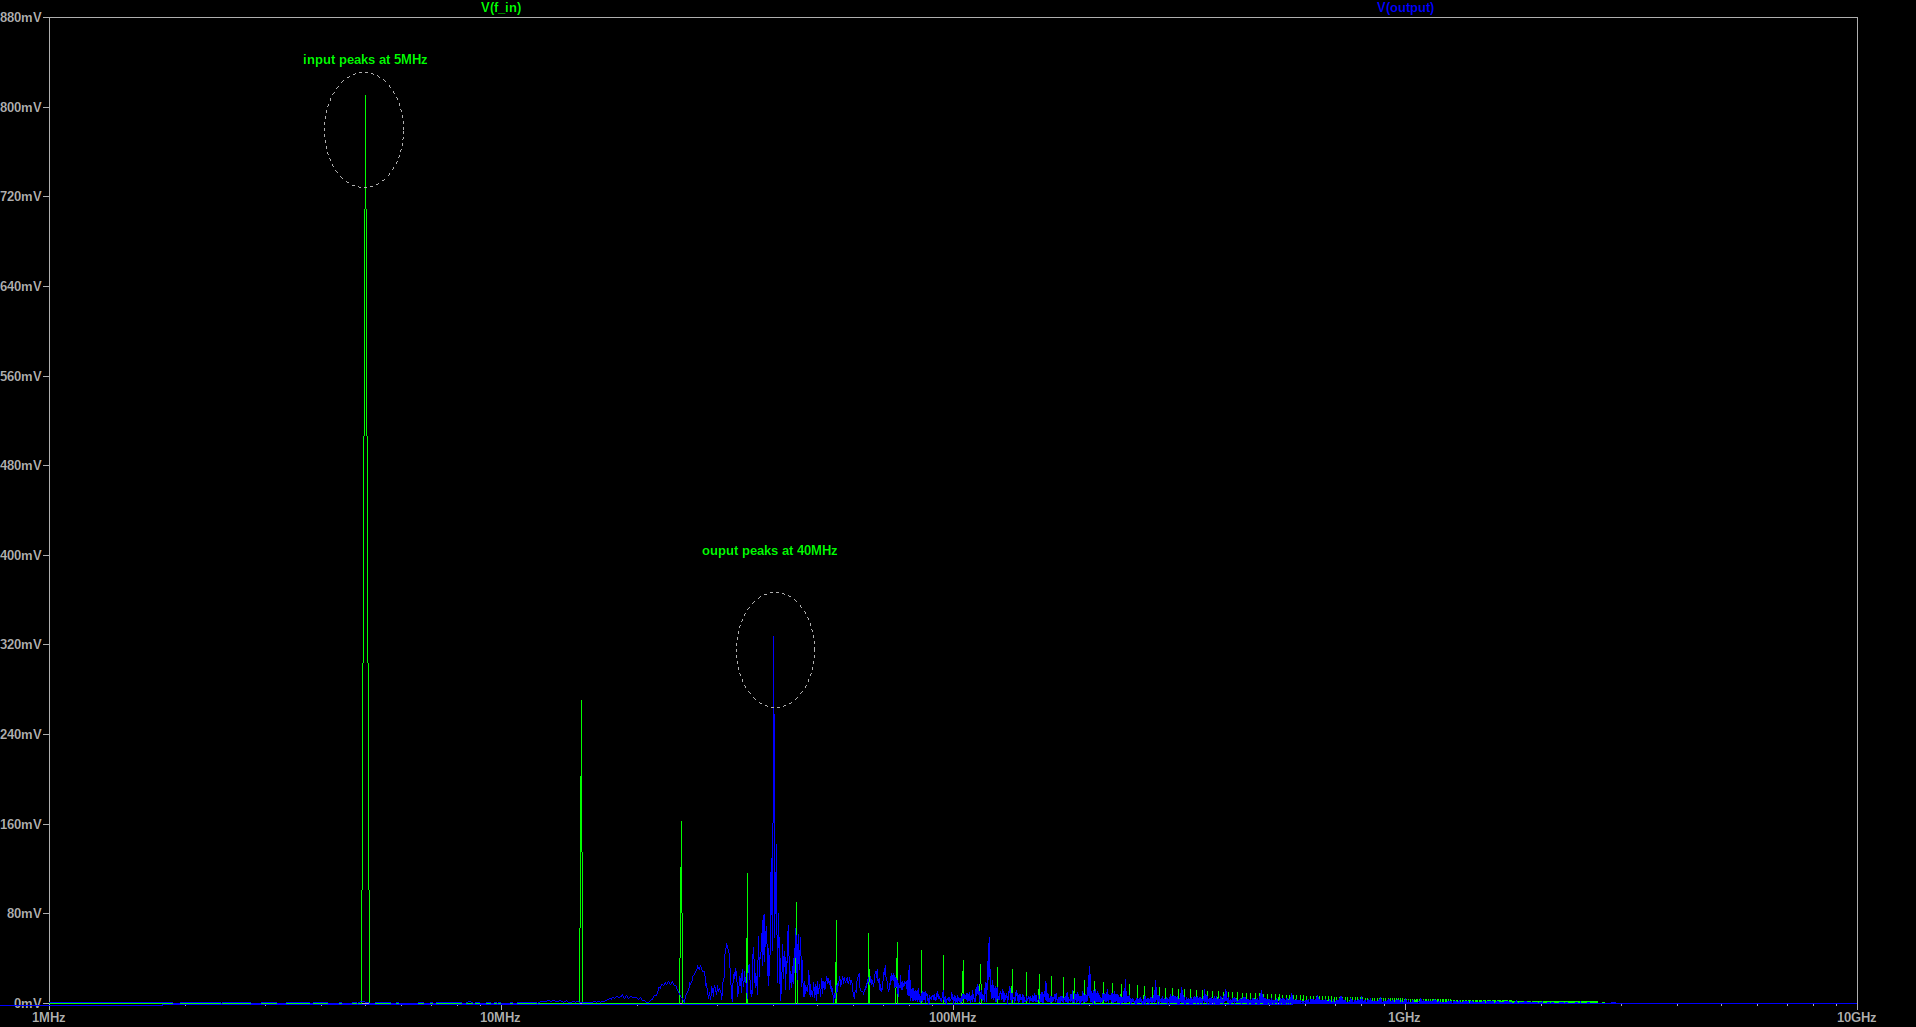
\includegraphics[width=1\linewidth]{figs/pllfftop2.png}
    \caption{Output Frequency Spectrum of PLL}
    \label{fig:output_frequency_spectrum}
    \vspace{0.5cm}
\end{figure}

Hence The following results were obtained from the simulation:
\begin{itemize}
    \item The output frequency is 40MHz, which is 8 times the input frequency of 5MHz.
    \item The output waveform is a square wave with a duty cycle of 50\%.
    \item The output amplitude is 1.8V, which is for whicht the VCO is designed for.
    \item The output frequency spectrum shows the frequency components of the output waveform, which are at 40MHz and its harmonics.
    \item Phase locking of the output waveform with the input waveform is observed.
\end{itemize}  

\section{Analysis}
Batch simulation was performed to analyze the performance of the circuit. The simulation was performed for different input frequencies. 
The input frequencies were varied from 1GHz to 500KHz. The output frequency was measured for each input frequency. The results of the simulation are shown in the following table \ref{tab:simulation_results}.

\begin{table}[H]
    \centering
    \begin{tabular}{|c|c|c|}
        \hline 
        \textbf{Simulation No.} & \textbf{Input Frequency} & \textbf{Output Frequency} \\
        \hline
        1 & 1GHz & --\\
        2 & 900MHz & --\\
        3 & 800MHz & --\\
        4 & 700MHz & --\\
        5 & 600MHz & --\\
        6 & 500MHz & --\\
        7 & 400MHz & --\\
        8 & 300MHz & --\\
        9 & 200MHz & --\\
        10 & 100MHz & --\\
        11 & 90MHz & --\\
        12 & 80MHz & --\\
        13 & 70MHz & --\\
        14 & 60MHz & --\\
        15 & 50MHz & --\\
        \hline
    \end{tabular}
    \caption{Simulation Results}
    \label{tab:simulation_results}
\end{table}
The output frequency was measured for each input frequency and observed through the ouput frequency Spectrum With respect to its input frequency spectrum achived through FFT view tool on LTSpice as shown in Figure \ref{fig:batch_input_frequency_spectrum} \& \ref{fig:batch_output_frequency_spectrum}.

Hence we can arrive to the conclusion the PLL able retain its functionality for the input frequency ranging from 22.5MHz to 3.75MHz.
\begin{figure}
    \centering
    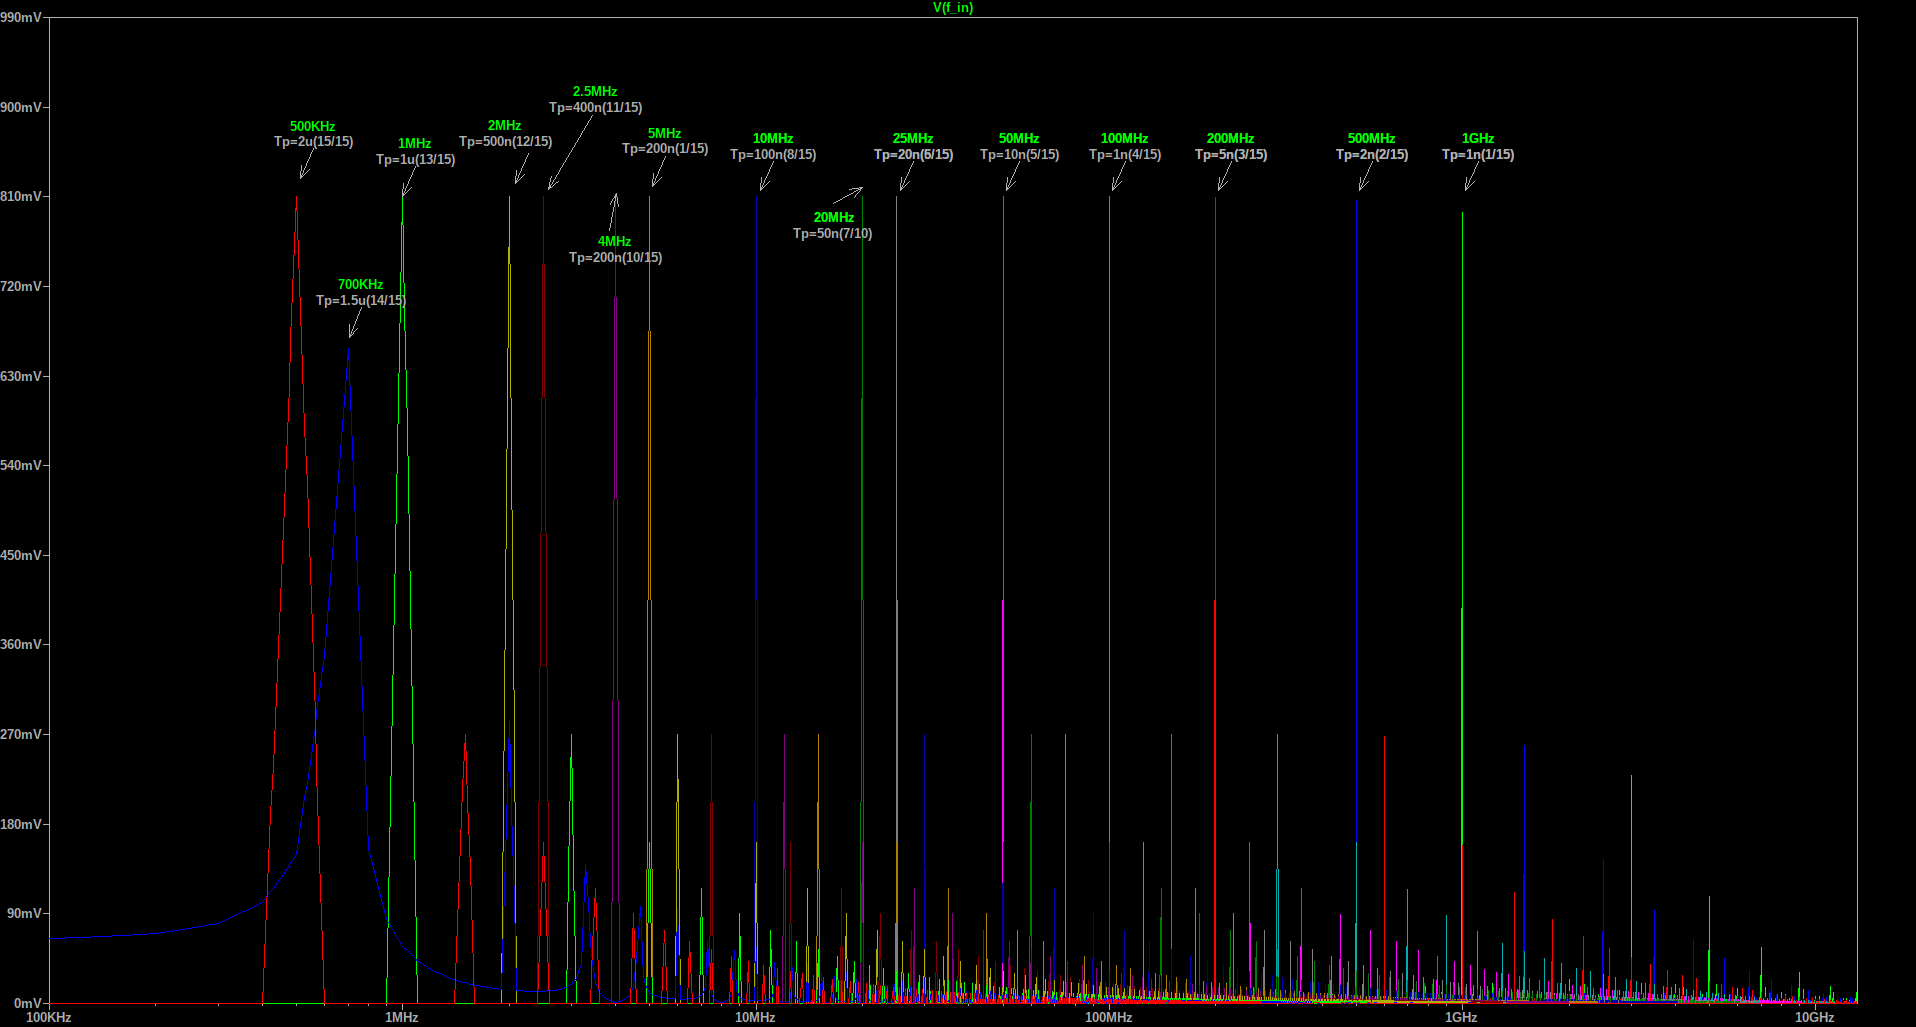
\includegraphics[width=1\linewidth]{figs/finfft.png}
    \caption{Output Frequency Spectrum of PLL}
    \label{fig:batch_input_frequency_spectrum}
    \vspace{0.5cm}

\end{figure}
\begin{figure}
    \centering
    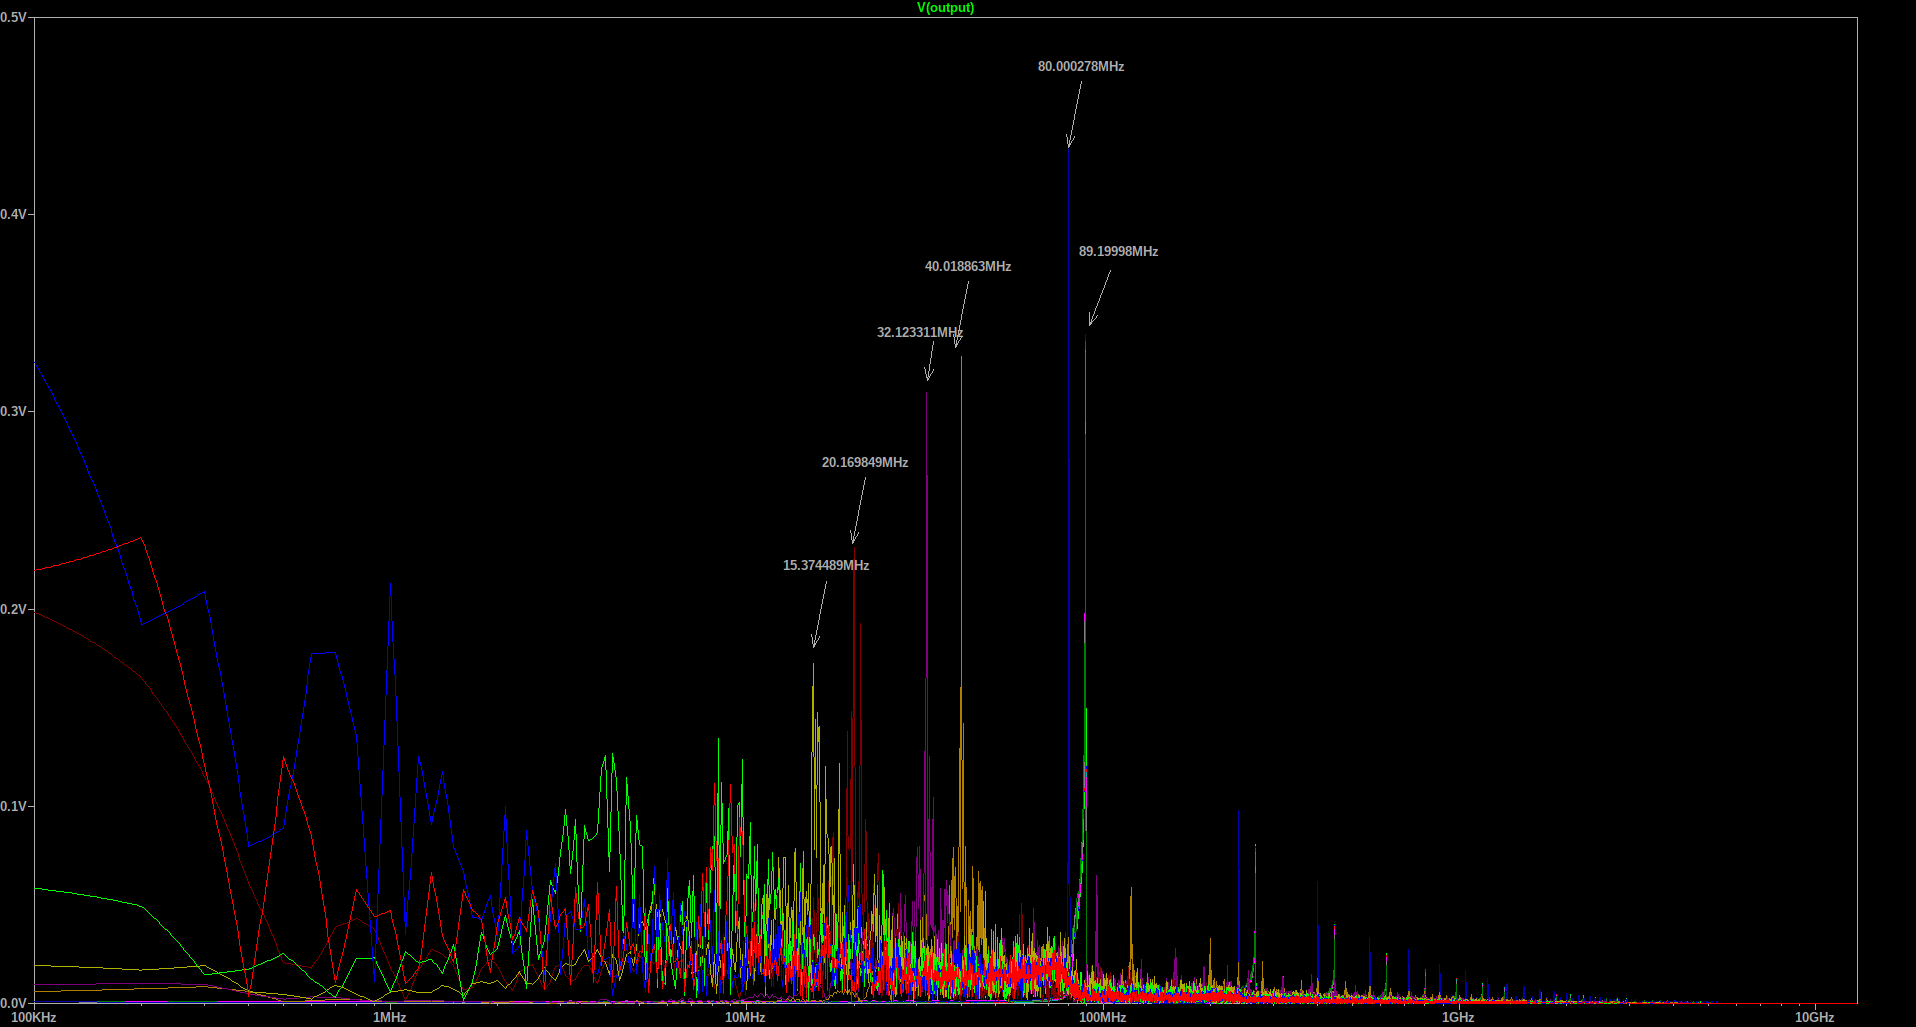
\includegraphics[width=1\linewidth]{figs/foutfft.png}
    \caption{Output Frequency Spectrum of PLL}
    \label{fig:batch_output_frequency_spectrum}
    \vspace{0.5cm}
\end{figure}